\documentclass[border=10pt]{standalone}
\usepackage{tikz}
\usetikzlibrary{shapes,arrows,positioning,shadows}

\begin{document}

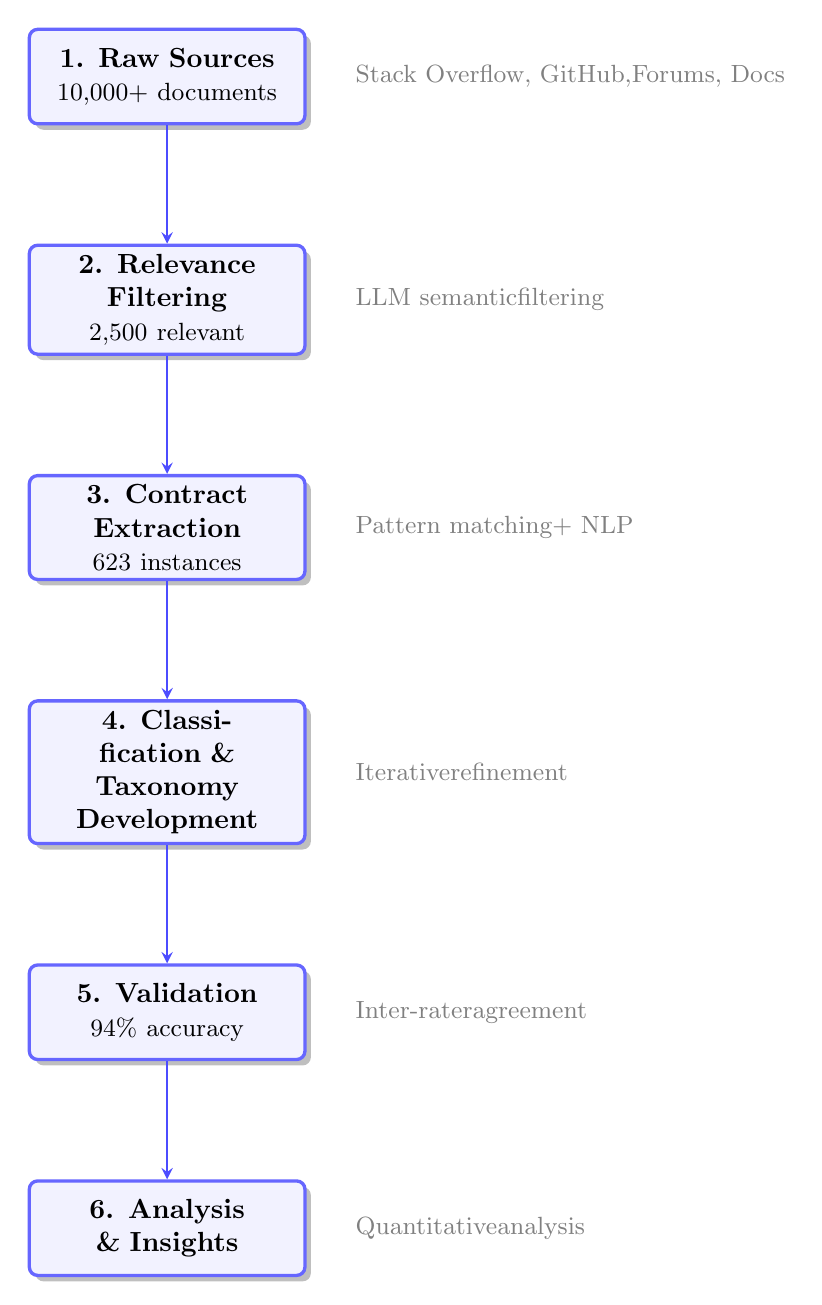
\begin{tikzpicture}[
    node distance=1.5cm,
    box/.style={
        rectangle,
        draw=blue!60,
        fill=blue!5,
        very thick,
        minimum height=1.2cm,
        minimum width=3.5cm,
        text width=3cm,
        align=center,
        rounded corners=3pt,
        drop shadow
    },
    arrow/.style={
        ->,
        thick,
        >=stealth,
        blue!70
    },
    label/.style={
        font=\small,
        text=gray
    }
]

% Stage 1
\node[box] (stage1) {
    \textbf{1. Raw Sources}\\
    \small 10,000+ documents
};

% Stage 2
\node[box, below=of stage1] (stage2) {
    \textbf{2. Relevance Filtering}\\
    \small 2,500 relevant
};

% Stage 3
\node[box, below=of stage2] (stage3) {
    \textbf{3. Contract Extraction}\\
    \small 623 instances
};

% Stage 4
\node[box, below=of stage3] (stage4) {
    \textbf{4. Classification \&}\\
    \textbf{Taxonomy Development}
};

% Stage 5
\node[box, below=of stage4] (stage5) {
    \textbf{5. Validation}\\
    \small 94\% accuracy
};

% Stage 6
\node[box, below=of stage5] (stage6) {
    \textbf{6. Analysis \& Insights}
};

% Arrows
\draw[arrow] (stage1) -- (stage2);
\draw[arrow] (stage2) -- (stage3);
\draw[arrow] (stage3) -- (stage4);
\draw[arrow] (stage4) -- (stage5);
\draw[arrow] (stage5) -- (stage6);

% Side annotations
\node[label, right=0.5cm of stage1] {Stack Overflow, GitHub,\\Forums, Docs};
\node[label, right=0.5cm of stage2] {LLM semantic\\filtering};
\node[label, right=0.5cm of stage3] {Pattern matching\\+ NLP};
\node[label, right=0.5cm of stage4] {Iterative\\refinement};
\node[label, right=0.5cm of stage5] {Inter-rater\\agreement};
\node[label, right=0.5cm of stage6] {Quantitative\\analysis};

\end{tikzpicture}

\end{document}
